\documentclass{article}
\usepackage{relsize}
\usepackage{tikz} % ,pgf,pgfarrows,pgfnodes,pgfautomata,pgfheaps,pgfshade}
\usetikzlibrary{shapes,decorations,shadings,positioning,arrows,snakes,3d}
\usepackage{amsmath,enumerate,xspace,subfig,siunitx}
\tikzstyle{legend} = [red, fill=white, font=\footnotesize, inner sep=2pt, rounded corners=0.05cm]
\tikzstyle{arrow} = [red, ->, line width=2pt]

\usepackage{amsmath,enumerate,xspace,subfig,siunitx,lscape}
\usepackage{listings}
\usepackage[absolute,overlay]{textpos}
\usepackage[colorinlistoftodos]{todonotes}

\usepackage[colorlinks=true,linkcolor=red,pagecolor=red,
  citecolor=blue,urlcolor=blue,breaklinks=true,
  hyperfootnotes=false,pdftitle={CombLayer Guide},
  pdfauthor={Stuart Ansell},pdfkeywords={CombLayer,MCNP,MCNPX}]
           {hyperref}
\renewcommand*{\rmdefault}{cmss} 


\definecolor{SlateBlue}{rgb}{0.1,0.1,1.00}
\definecolor{SlateGreen}{rgb}{0.1,0.8,0.3}
\definecolor{darkred}{rgb}{0.8,0,0}
\newcommand{\tcg}[1]{
   \textcolor{green}{#1}}
\newcommand{\tcr}[1]{
   \textcolor{red}{#1}}
\newcommand{\tcb}[1]{
   \textcolor{blue}{#1}}
\newcommand{\tcbb}[1]{
   \textcolor{SlateBlue}{#1}}
\newcommand{\tcgg}[1]{
   \textcolor{SlateGreen}{#1}}


\definecolor{mygray}{rgb}{0.4,0.4,0.4}
\definecolor{mygreen}{rgb}{0,0.8,0.6}
\definecolor{myorange}{rgb}{1.0,0.4,0}

\lstset{
  basicstyle=\small\sffamily\color{black},
  commentstyle=\color{red},
  frame=false,
  numbers=left,
  numbersep=5pt,
  numberstyle=\tiny\color{mygray},
  keywordstyle=\color{blue},
  showspaces=false,
  showstringspaces=false,
  stringstyle=\color{myorange},
  tabsize=8,
  otherkeywords={std},
  escapeinside={\%\%}{\@},
  xleftmargin=0.0\linewidth
}
\newcommand {\prog}[1]{{\it #1}}
\newcommand {\vb}[1]{\begin{\verbatim}{#1}\end{verbatim}}
\newcommand {\alert}[1]{\textcolor{red}{#1}}
\lstnewenvironment{bash}{\lstset{language=bash,numbers=none,backgroundcolor=\color{yellow!20},frame=tb}}{}
\lstnewenvironment{cpp}{\lstset{language=C++,numbers=none,backgroundcolor=\color{green!10},frame=tb}}{}
\lstnewenvironment{deck}{\lstset{language=bash,numbers=none,backgroundcolor=\color{gray!10},frame=tb}}{}
\lstnewenvironment{xml}{\lstset{language=xml,numbers=none,backgroundcolor=\color{green!10},frame=tb}}{}

\setlength{\parindent}{0in}
\setlength{\parskip}{0.1in}
\setlength{\textwidth}{6.5in}
\setlength{\textheight}{9.0in}
\setlength{\oddsidemargin}{0.0in} 
\setlength{\evensidemargin}{0.0in} 

\newcommand{\mcnp}{{\tt MCNP}\xspace}

\newcommand{\figref}[1]{Fig.\,\ref{#1}}
\newcommand{\figrefp}[1]{Fig.\,\ref{#1} on page~\pageref{#1}}

\newcommand{\secref}[1]{Sec.\,\ref{#1}}
\newcommand{\secrefp}[1]{Sec.\,\ref{#1} on page~\pageref{#1}}

\newcommand{\git}[1]{\marginpar{Git hash:\\ \href{http://github.com/SAnsell/CombLayer/commit/#1}{#1}}}


\newcommand{\xangle}{15}
\newcommand{\yangle}{153}
\newcommand{\zangle}{90}
\newcommand{\xlength}{1}
\newcommand{\ylength}{1}
\newcommand{\zlength}{1}
\pgfmathsetmacro{\xx}{\xlength*cos(\xangle)}
\pgfmathsetmacro{\xy}{\xlength*sin(\xangle)}
\pgfmathsetmacro{\yx}{\ylength*cos(\yangle)}
\pgfmathsetmacro{\yy}{\ylength*sin(\yangle)}
\pgfmathsetmacro{\zx}{\zlength*cos(\zangle)}
\pgfmathsetmacro{\zy}{\zlength*sin(\zangle)}
\newcommand{\dimension}{3}% actually dimension-1
\newcommand{\dimensionZ}{7}% actually dimension-1

\newcommand{\drawMug}[3]{
  \def\width{4};
  \def\height{5};
  \coordinate (A) at (#1,#2);
  \coordinate (B) at (#1+\width,#2+\height);
  \draw[#3] (A) rectangle (B);
  \draw[#3] (#1,3) arc (90:270:1cm);
  \draw[#3] (#1,3.3) arc (80:280:1.3cm);
}

\newcommand{\drawSpoon}[3]{
  \def\hWidth{0.5};
  \def\hHeight{5};
  \def\lWidth{0.3};
  \def\lHeight{1.5};
  % ladle
  \coordinate (C) at (#1-\lWidth,#2);
  \coordinate (D) at (#1+\hWidth+\lWidth,#2+\lHeight);
  \draw[#3] (C) rectangle (D);
  % handle
  \coordinate (A) at (#1,#2+\lHeight);
  \coordinate (B) at (#1+\hWidth,#2+\hHeight);
  \draw[#3] (A) rectangle (B);
}


\title{CombLayer Guide}
\author{Stuart Ansell}

\usepackage{nomencl}
\makenomenclature

\begin{document}
\maketitle
\tableofcontents
\clearpage
\printnomenclature[2cm]
\clearpage


\section{Introduction}

CombLayer is designed to facilitate the rapid production of complex
MCNPX models that depend on a long list of ranged variables and a
number of module flags. It is also intended to help with placement of tallies,
maintaining consistant material files and some variance reduction.

\subsection{Coding Convensions}

CombLayer has some coding convensions beyond the standard Scott Meyers:
{\it Effective C++} conventions \cite{Meyers}. These are typcially their for
two reasons (i) the in a model-build system rapid build time is
essential since it is impossible to have a sub-test framework for any
component as the whole MCNPX model is required to check if is it
valid, (ii) the code is intended to be used without complete
understanding. Therefore as much as possible, each component is
independent without code repetition. Akk back-references are to be minimized
both in the run-time calling path and in the code build dependencies.

\subsubsection{Include files}
\label{Sec:IntroInclude}
 Include files (.h) are forbidden to include other
files. This does several things (a) it reduces the {\it dependency
  hell} where it is almost impossible to find the definition of a
function and what it depends on. (b) optimization of the include tree
can be carried out and dependency continuously observered. 

Namespaces are a good method of removing global name pollution but
many other C++ programs allows {\it using namespace X} this is almost
100\% forbidden except in the test for that particular namespace
unit. This also applies to boost, stl, tr1 etc, to which helps
distinguish external functions and domains.



\newpage
The basic program structure is given by figure \ref{MainLayout}.  The
main program structure is normally copied from an existing project and
the areas are constructed by the user. It is normal to add inputs
(from the command line), variables that your project is going to use,
and then build the geometry constructor via a call to a makeProject
command.  There are other ways to construct the system but this allows
a degree of autonomy from tallies/variance reduction and producing an
appropiate output.

\begin{figure}[!htp]
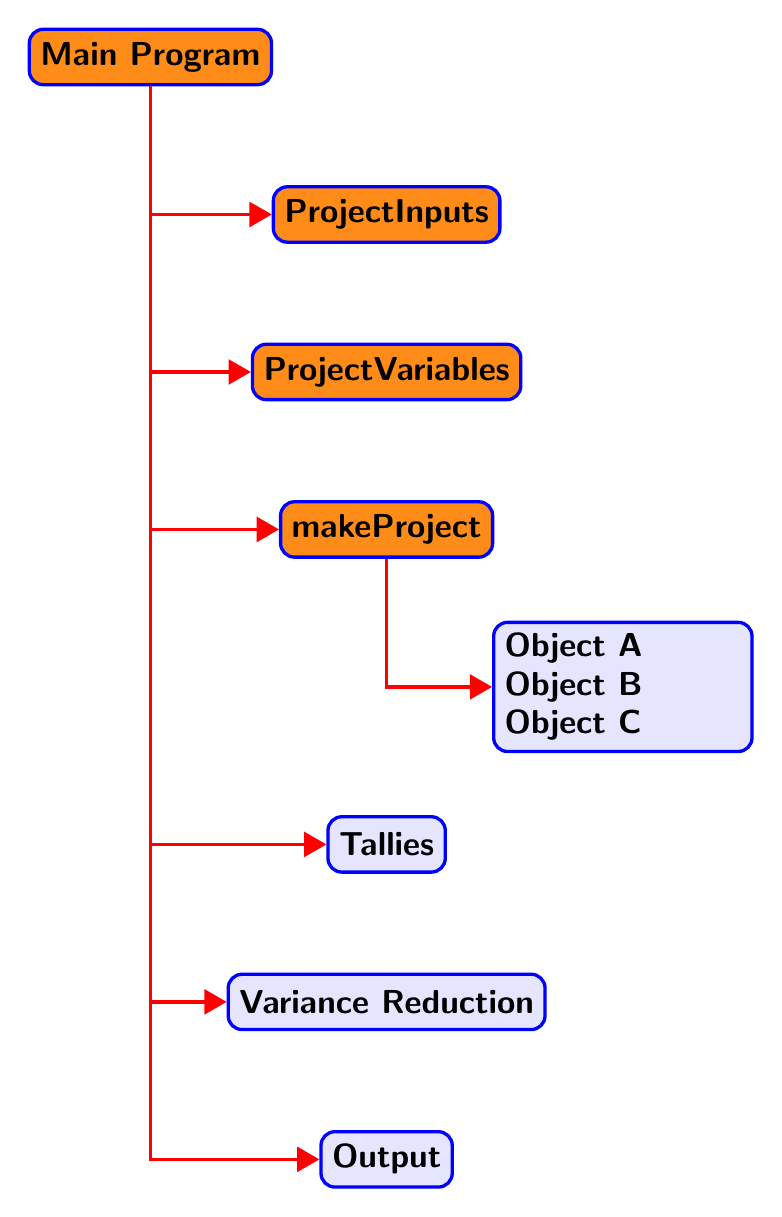
\begin{tikzpicture}

  \coordinate (Main) at (0,0);
  \coordinate (Input) at (3,-2);
  \coordinate (Var) at (3,-4);
  \coordinate (Project) at (3,-6);
  \coordinate (Object) at (6,-8);
  \coordinate (Tally) at (3,-10);
  \coordinate (Variance) at (3,-12);
  \coordinate (Output) at (3,-14);

  \tikzstyle{fbox}=[draw=blue,very thick,
                    shape=rectangle,rounded corners=0.5em,
                    inner sep=4pt,
                    minimum height=2em,text badly centered,
                    fill=orange!90!white];
  \tikzstyle{obox}=[draw=blue,very thick,
                    shape=rectangle,rounded corners=0.5em,
                    inner sep=4pt,
                    minimum height=2em,text badly centered,
                    fill=blue!10];

%  \draw[blue,line width=0.4mm,->] (tally) (tally) -- (weight);
%  \draw[blue,line width=0.4mm,->] (tally) (geom) -- (weight);
%  \draw[blue,line width=0.4mm,->] (tally) (var) -- (geom);
%  \draw[blue,line width=0.4mm,dashed,->] (tally) -- (geom);


  \node[fbox] (MainBox) at (Main) { \bf \large Main Program } ;

  \node[fbox] (InputBox) at (Input) { \bf \large ProjectInputs };
  \draw[->,very thick,color=red,>=triangle 60] (MainBox) |- 
                   node[left]{} (InputBox) ;

  \node[fbox] (VarBox) at (Var) { \bf \large ProjectVariables };
  \draw[->,very thick,color=red,>=triangle 60] (MainBox) |- 
                   node[left]{} (VarBox) ;

  \node[fbox] (ProjectBox) at (Project) { \bf \large makeProject };
  \draw[->,very thick,color=red,>=triangle 60] (MainBox) |- 
                   node[left]{} (ProjectBox) ;

  \node[obox] (ObjectBox) at (Object) { \parbox{3.0cm}{ \bf \large Object A\\
 Object B\\ Object C} };
  \draw[->,very thick,color=red,>=triangle 60] (ProjectBox) |- 
                   node[left]{} (ObjectBox) ;

  \node[obox] (TallyBox) at (Tally) { \bf \large Tallies };
  \draw[->,very thick,color=red,>=triangle 60] (MainBox) |- 
                   node[left]{} (TallyBox) ;

  \node[obox] (VarianceBox) at (Variance) { \bf \large Variance Reduction };
  \draw[->,very thick,color=red,>=triangle 60] (MainBox) |- 
                   node[left]{} (VarianceBox) ;

  \node[obox] (OutputBox) at (Output) { \bf \large Output };
  \draw[->,very thick,color=red,>=triangle 60] (MainBox) |- 
                   node[left]{} (OutputBox) ;
\end{tikzpicture}
\caption{The main program calling sequence is shown. The parts
  in orange, are expected to be constructed by the user. Bespoke objects
  can be added for a project but it is not necessary.  }
\label{MainLayout}
\end{figure}


\subsection{Main}

The main function for CombLayer follows a relatively linear template.
Consider the example

\begin{lstlisting}[language=C++]{Name=MainProg}{floatplacement=H}

int 
main(int argc,char* argv[])
{
  int exitFlag(0);                // Value on exit
  ELog::RegMethod RControl("","main");
  mainSystem::activateLogging(RControl);
  std::string Oname;
  std::vector<std::string> Names;  
  std::map<std::string,std::string> Values;  

  // PROCESS INPUT:
  InputControl::mainVector(argc,argv,Names);
  mainSystem::inputParam IParam;
  %%{\tcgg{\bf createPipeInputs(IParam);}@

  Simulation* SimPtr=createSimulation(IParam,Names,Oname);
  if (!SimPtr) return -1;

  // The big variable setting
  %%{\tcgg{\bf setVariable::PipeVariables(SimPtr-$>$getDataBase());} @
  InputModifications(SimPtr,IParam,Names);
  
  // Definitions section 
  int MCIndex(0);
  const int multi=IParam.getValue<int>("multi");
  try
    {
      SimPtr->resetAll();
      
     %%{\tcgg{\bf pipeSystem::makePipe pipeObj;}@

      World::createOuterObjects(*SimPtr);
     %%{\tcgg{\bf pipeObj.build(SimPtr,IParam)}; @  
      SDef::sourceSelection(*SimPtr,IParam);
      
      SimPtr->removeComplements();
      SimPtr->removeDeadSurfaces(0);         
      ModelSupport::setDefaultPhysics(*SimPtr,IParam);
      
      const int renumCellWork=tallySelection(*SimPtr,IParam);
      SimPtr->masterRotation();
      if (createVTK(IParam,SimPtr,Oname))
	{
	  delete SimPtr;
	  ModelSupport::objectRegister::Instance().reset();
	  ModelSupport::surfIndex::Instance().reset();
	  return 0;
	}
      
      if (IParam.flag("endf"))
        SimPtr->setENDF7();
      
      SimProcess::importanceSim(*SimPtr,IParam);
      SimProcess::inputPatternSim(*SimPtr,IParam); // energy cut etc
      
      if (renumCellWork)
	tallyRenumberWork(*SimPtr,IParam);
      tallyModification(*SimPtr,IParam);
      
      if (IParam.flag("cinder"))
	SimPtr->setForCinder();
            
      // Ensure we done loop
      do
	{
	  SimProcess::writeIndexSim(*SimPtr,Oname,MCIndex);
	  MCIndex++;
	}
      while(MCIndex<multi);
      
      exitFlag=SimProcess::processExitChecks(*SimPtr,IParam);
      ModelSupport::calcVolumes(SimPtr,IParam);
      ModelSupport::objectRegister::Instance().write("ObjectRegister.txt");
    }
  catch (ColErr::ExitAbort& EA)
    {
      if (!EA.pathFlag())
	ELog::EM<<"Exiting from "<<EA.what()<<ELog::endCrit;
      exitFlag=-2;
    }
  catch (ColErr::ExBase& A)
    {
      ELog::EM<<"EXCEPTION FAILURE :: "
	      <<A.what()<<ELog::endCrit;
      exitFlag= -1;
    }
  %%{\it delete SimPtr;} @
  ModelSupport::objectRegister::Instance().reset();
  ModelSupport::surfIndex::Instance().reset();

  return exitFlag;
}
\end{lstlisting}

The Main program given in listing \ref{MainProg} highlights the areas
that the user should be creating. The remainder of the main() function
deals with trapping exceptions, loggin and building variance reduction
and tallies into the model.

\begin{enumerate}[(i)]
\item {\bf createPipeInputs} is a 
function to define which command line options [above the standard ones]
this model should support. It doesn't do anything with them, just a
list of options, number of arguements they can take and any default
values that the options should take. All options defined here are
access from the command line option with a {\it -} sign. E.g. {\it -r} as a
renumber operation. In this form of the program, if the main program
is run without any options, a list and very brief description of each
option is shown (e.g. execute {\it ./pipe}).

If no additional options are required, a call to
{\it createInputs(IParam)} would be expected. Significant restructuring
would need to take place to avoid that call.
\item \tcgg{setVariable::PipeVariables} is the method that registers
and sets a default value for all the variables that the model will
use. 
\item \tcgg{makePipe pipeObj} and \tcgg{pipeObj.buid(SimPtr,IParam)} are the
main geometry building calls. Typically 100\% of the geometry is built
in this zone. It is not a place for tallies, variance reduction and other
non-geometry items.
\end{enumerate}




\section{Installation}

CombLayer is predominately written for the Linux platform using {\tt C++}
compilers that support {\tt C++11} or greater. The code is available from \\
\href{https://github.com/SAnsell/CombLayer}{https://github.com/SAnsell/CombLayer}, \\ either as a download of a {\tt zip} file or
by cloning/pulling the git repository.

\subsection{Requirments}

CombLayer needs to have the GNU Scietific Library [GSL] and the
{\tt boost::regex} system along with the STL libraries from your {\tt C++}
compiler. The GSL can be avoided with the {\tt -NS} flag in the {\tt getMk.pl} \checkme{or CMake.pl?} script
but some functionality will be lost, particularly in the choice
of variance reduction methods.

Additionally, the primary build system uses {\tt cmake}. There is another
that just uses {\tt make} but is significantly more time-consuming.

Functional documentation is supported using {\tt Doxygen} and the construction
of new cmake text files can be done via PERL scripts.

Currenly it is know that {\tt gcc} version 4.6 and above can compile
CombLayer as can {\tt clang} (all tested versions). {\tt gcc} 4.4 which is often
the default on RedHat systems (2015) does not work.

\subsection{Basic build method}

If a clean directory is made and then the {\tt .zip} file is uncompressed, the
following commands should build a version of CombLayer.

\begin{bash}
  ./CMake.pl
  cmake ./
  make
\end{bash}

This should make a number of executables, e.g. {\tt ess}, {\tt simple}, {\tt fullBuild} etc. These
can be used to make a simple model with commands like
\begin{bash}
  ./simple -r AA
\end{bash}
This will produce an output file {\tt AA1.x} which is a MCNP model.




\section{Link system}

CombLayers geometry is composed of a set of objects that have slightly
stronger rules than a typical MCNPX model. Obviously any MCNPX model
can be represented as a CombLayer model and in the extreme case that
is done by defining one object to contain the MCNPX model. However, the
little benefit would be derived from such an approach.

The basic geometric system is to build a number of geometric classes
and construct the model by incorporating those into the desired
configuration. Each geometric class is designed to be built and an
arbitary position and rotation, be of an undetermined number, and
interact with its surroundings in a well defined manor. 

In object orientated programming, functional rules and properties are
normally added to objects by inherritance. CombLayer follows that
pattern. As such most geometry item classes inherit from base classes within 
the {\tt attachSystem} namespace.

\subsection{AttachSystem Namespace}
\label{AttachSystem}

The CombLayer system is built around the interaction of FixedComp
units, ContainedComp units and LinkUnits. The use of these and their
interactions are the basic geometric building tools. These object
reside within the attachSystem namespace.

Almost any geometric item can be designated as a FixedComp
object. This is done by public inherriting from directly from the
FixedComp, or by inherriting from one of the more specialised attachSystem
objects e.g. TwinComp or LinearComp. 

\subsection{FixedComp}

The basic FixedComp object holds the origin and the orthoganal basis
set (X/Y/Z) for the geometry item being built. In addition it holds a 
number of LinkUnits which provide information about the outer (and/or inner)
surfaces and positions on the geometric item. 

As with all Object-Orientated (OO) constructions their is an implicit
contract that the inherited object should adhere to. This is normally
expressed as the {\it Liskov Substitution principle}: This principle
states that functions that use pointers/references to the base object
must be able to use the objects of derived classes without knowing
it. In this case, that means that modification of the origin or the
basis set should not invalidate it and that the object should do the
expected thing. E.g. if the origin is shifted by 10 cm in the X
direction the object should move by 10cm in the X direction. It also
means that the basis set must remain orthogonal at all time.

Other than providing an origin and an basis set, the FixedComp has a
number of link points. The link points are there to define joining
surfaces, points and directions. Each link point defines all three parts.

For example a cube might have 6 linkUnits, and each linkUnit would
have a point at the centre of a face, a direction that is normal to
the face pointing outwards and a surface definition that is the
surface pointing outwards. \[ Note that in the case that the link
points define an inner volume, for example in a vacuum vessel, then
the surfaces/normals should point towards the centre.\]

The actual link surface does not need to be a simple surface. In the
case, that an external surface needs multiple surfaces to define the
external contact these can be entered into a link-rule. For example,
if the cube above was replaces with a box with two cylindrical
surfaces the link surface would be defined as the out going cylinder
intersection with a plane choosing the side. 

In the case of an equiry for the linkSurface (e.g. to do an line
intersection) then it is the first surface that takes
presidence. However, all actions can be carried out on the link-rule
including line intersections etc.


\subsection{ContainedComp}

The ContainedComp defined both the external and interal enclosed
volume of the geometric item. It is most often used to exclude the
item from a larger enclosing geometric object: e.g. A moderator will
be excluded from a reflector, or it can be used to exclude a part of
the geometric item from another geometric object. E.g. two pipes which
overlap can have one exclude itself from the other. 

In CombLayer, the ContainedComp are considered the primary geometric
item, i.e. it is the ContainedComp that is removed from the other
items.  However, it is used in a two stage process wereby cells are
registered to be updated by the ContainedComp at a later date. This
was to allow forward dependency planning but has more or less been
superseded by the attachControl system.


\section{Model Runtime control}

C++ programs start from the main() function and in CombLayer the
runtime control has been keep mostly in the main() function. Clearly
that could be further refactored out but CombLayer lacks the
sophisticated top level type abstraction that is required to do this
in a generic way, so copy/pasted structure is used with variance to
the particular model required. The sole advantage of the abscence of a
top level abstraction is that the user is the freedom in writing new objects
which allows other programs to be incorporated by making their main function
a minor function and directly calling.

The structure of two example main()s will be compared from the units
that exist with the stanard CombLayer distribution. That is {\it
bilbau.cxx} and {\it reactor.cxx}. These build the delft reactor model and the
Biblau low energy spallation source.

First part of the code is along list of \#include's. They are the
mainly dependency list of the objects {\it Simulation, weightManager,
and tallySelector.} This can and should be copied at will. Do not
make an file with them all in [see \ref{Sec:IntroInclude}].

At the end of the include section there is typically, one or two model
specific includes. These normally include {\it makeXXX.h} file and
anything that they directly depend on. In the case of bilbau it is just 
{\it makeBib.h} whilst for reactor it is both {\it makeDelft.h} and \prog{ReactorGrid.h}.

\subsection{makeModel}

The makeModel object is the place that creates, initializes and
manages inquires for the instances of all the geometric components. 
Primary objects need to be created and registered with the objectRegister 
\ref{objectRegister}. The makeModel component is 
 




Tallies are the fundamental reason for running MCNPX. However, the
manor in which MCNPX specifies tallies is not compatible with a
vairiable defined model because in most cases the required tally is relative 
to an object whose position is unknown. 

This problem has been addressed by allowing most tallies to use the 
FixedComp link system. 

\subsection{Tally System}

The tally system is accessed either by a simple command line menu
system, or via an XML file. The command line help system is very
primative but can remind the user of the bais

\subsection{Point Tally}
\label{PointTally}

Point tallies are fundamentally a 3D vector in space. In CombLayer,
there are three levels of position available: (a) Real MCNPX output
position, (b) CombLayer master origin position before master rotation,
and (c) relative position to an object. Both (a) and (c) are well
supported, however, to do option (b) there needs to be some real care
with the layout of the calling sequence in the main() function. The
fullBuild.cxx example is a suitable option to follow, but checking
will be needed.

As

%\section{HowTo}
\begin{itemize}
\item Get real surface number by its relative number: SMap.realSurf(divIndex+103) (see createLinks methods)
\end{itemize}

\subsection{How to put one object into another}

Suppose, we are inserting Spoon into Mug.
Mug is made up of N cells. Spoon is made of one contained component with outer surface.
CombLayer provides several methods to put one object into another:

\begin{cpp}{Name=essBuild}{floatplacement=H}
attachSystem::addToInsertForced(System,   *Mug, *Spoon);
attachSystem::addToInsertSurfCtrl(System, *Mug, *Spoon);
attachSystem::addToInsertControl(System,  *Mug, *Spoon);
attachSystem::addToInsertLineCtrl(System, *Mug, *Spoon);
\end{cpp}

\subsubsection{addToInsertForced}

The outer surface of the Spoon is excluded from the HeadRule of every single cell of Mug.
Even if Mug contains cells which do not intersect with Spoon (e.g. its handle, see \figref{fig:forced}).
{\it Forced} means {\it do it and do not think about it}, but at the same time it means that
{\it I have got something wrong somewhere.}  Normally this is that insufficient link points have been added
to the object, or that the object is a set of split (single cell) volumes.  However, there is the additional
problem that the model may not be correctly constructed at this point, so that the other options seem not to work.
This can be checked by adding a
\prog{SimProcess::writeIndexSim(System,"OutputFilename.txt",0);}
in the code just before the call to insertForced. If there are undefined volumes then the model is not in a state that
any of the \prog{addToInsert} algorithms except \prog{addToInsertForced} can be used. 

\begin{figure}
  \centering
  \begin{tikzpicture}
    \drawMug{0}{0}{}
    \drawSpoon{2}{1}{dashed}
  \end{tikzpicture}
  \caption{addToInsertForced: all cells of Spoon are excluded from all cells of Mug including non intersecting cells}
  \label{fig:forced}
\end{figure}


\subsubsection{addToInsertSurfCtrl}

The objective of this function is to use the surface intersections between Mug and spoon to determine which 
cells within Mug intersect the ContainedComp of spoon. The process is done on a cell - ContainedComp level. 

The process is as follows:
\begin{enumerate}

\item{Deconvolves both the Spoon's containedComponent boundary into surfaces.}
\item{Loop over each cell in Mug : MCell}
  \begin{enumerate}
  \item{Calculate intersection of each surface:surface:surface triplet from the set of CC surfaces and MCell surface}
  \item{If a point is within CC and the MCell exclude the CC from the
    MCell and goto next cell}
  \end{enumerate}
\end{enumerate}
   
Thus the spoon is inserted only into those cells of Mug which it intersects.

It is not always better to call {\tt addToInsertSurfCtrl} instead of
{\tt addToInsertForced} in cases that if is certain that an
intersection can must take place (particularly if the CC / Inserting
cells have large numbers of surfaces).

{\tt addToInsertSurfCtrl} is a very expensive function to call,
because you have to check all the surface triplets. So, it runs a bit
slower than addToInsertForced, but the geometry will be faster.  The
two remaining methods provide similar functionality but with less
computational overhead, however, there are cell constructs which will
cause them to fail.

\subsubsection{addToInsertControl}

It's a very simple method. The link points from Spoon are uses as a test for each of the cells within Mug. 
The method checks if any of these link point fit inside each of the cells of Mug. If it does, then it cuts Spoon from the Mug cell.
It is possible to add a vector of link points to check as a parameter to limit the search.

\subsubsection{addToInsertLineCtrl}

Imagine we have a (big) contained component~(Mug) and some (small)
object which clips it~(Spoon). The link points are {\bf not} in the
Mug~(therefore {\bf addToInsertControl} can not be used), but the
lines which connect them are in the Mug.  The method checks the lines
connecting the link points and sorts out the intersections.


\section{Components}

\subsection{ObjectRegister}
\label{ObjectRegister}

The objectRegister is a singleton object [it should be per
  simulation], which keeps each and then deletes when at its lifetime
end, each object registered with it. It only accepts two types of
object, a dummy name object and a FixedComp object. 

If a dummy object is required, the name (and possibly number) of the object 
is provided and the objectRegister singleton provides a unique
range of cell and surface numbers, typically 10,000 units of each, but
can be user selected. This is its only responsibility and to ensure that the
name is unique. 

Significantly more complex is the FixedComp registration, in this case
a \prog{std::shared\_ptr} of FixedComp must be provided by the
calling method. Obviously, for a shared\_ptr the object memory must be
allocated, i.e. an initial \verb|new object(...)| is normally called
directly or previously. A typical structrue might be:

\begin{verbatim}
std::shared_ptr<BeamPipe> A 
   = new BeamPipe("LongPipe");

ModelSupport::objectRegister& OR=
    ModelSupport::objectRegister::Instance();

OR.addObject(A);
\end{verbatim}

From this example, the BeamPipe class is inherrited from FixedComp,
this is manditory. A tempory reference \prog{OR} is created by calling
the static Instance() method. All singletons in CombLayer provide an
Instance() method for this purpose. Then the object pointer is referenced
to the objectRegiste with \prog{addObject}.

However, hidden from view is a call to objectRegister in FixedComp's
constructor, which is certain to be called as all registered object must derive
from this class. That occures during the operator new call and results
in the allocation of the cell/surface numerical range. If it is
necessary to trap that error, the try/catch block must be around the
new opertor. The main exception that is possible if an existing object
already exists with the same name.




\subsection{EXT Command}
\label{ExtCommand}

MCNP(X) provides the EXT card for biasing the direction of the
particles after collisions. The card can be configured with a
stretching parameter value between -1.0 and 1.0 and an optional vector
or direction associated with it. If a vector is not given the
stretching parameter is applied in the direction of the neutron travel.

MCNP(X) only accepts the direction to be X,Y,Z which is highly
limiting in the CombLayer environment, so it is only partially supported.

The other two options vector and non-vector are supported.

\subsection{-wExt entry}

The first method of entry is via the command line option -wExt. This
command takes a sequence of additional values which are split into a
{\it zone} and {\it type} region. The {\it zone} region is based on
the cells that are to be biased. This can be give with the commands:

\begin{itemize}
\item{ {\bf all} : Apply to all non-void cells}
\item{ {\bf Object [name]} : Apply to all objects within the object name}
\item{ {\bf  Cell [Range]} : Apply to all objects within the range  }
\end{itemize}

Name can be a compound name of type objectName:CellMapName. This would
just select those cells within the cellMap unit of the particular
object.

The type


\section{User guide}
This section describes how to use CombLayer from a user's (i.e. non-developer) point of view.
In this guide, it is assumed that the user has no C++ or coding experience.

The guide is focused on the ESS model, which can be generated by running. 
\begin{bash}
  ./ess -r modelOut
\end{bash}
This command produces the \mcnp input file {\tt modelOut1.x} as well as two other files: {\tt ObjectRegister.txt} and {\tt Renumber.txt}.

The single flag {\tt -r} is optional for MCNP6 as it causes the objects and surfaces in MCNP to be renumbered sequentially and
to fit within the 100,000 object/surface limits of MCNPX.

\subsection{Variables}
In the beginning of the input file there is a commented list of variables which define the geometry:

\begin{deck}
 c ----------------------------------------------
 c --------------- VARIABLE CARDS ---------------
 c ----------------------------------------------
 c ABunkerFloorDepth 120
 c ABunkerFloorThick 100
 c ABunkerLeftAngle 0
 c ABunkerLeftPhase -65
 c ABunkerNLayers 1
 ...
\end{deck}

The variable name consists of the component name and its corresponding parameter. For instance,
the first variable {\tt ABunkerFloorDepth} in the list above sets the floor depth of the component called {\tt ABunker}.

Only variables that have needed to be examined are included in this output. Several components are optional and if not built then
their corresponding variables are not seen in the output. All variables start with an initial value and stateless variables are prohibited.
Most variables are defined appropiately within the CombLayer program and obviously can be changed by editing the code and recompiling.
However for a simple variable change that is excessive work so there are a number of methods to change variables from the command line.

\subsubsection{How to change variables}
Any of these variables can be changed either via a command line arguments or an XML file.

As an example, consider changing the Beryllium reflector height.
First of all, we need to find out which variable we need to change and therefore find out the name of the Be reflector
component in CombLayer.

To do this, open the \mcnp geometry and click on any Be reflector cell. Currently, it's cell number 5~(exact number depends on the
CombLayer version you are using).

Now we need to find out which component this cell belongs to.  Find this cell number in the {\tt Renumber.txt} file:
\begin{bash}
grep " 5 " Renumber.txt 
Surf Change:1000006 5                                                           
Cell Changed :1000005 5 Object:BeRef (topBe)       
\end{bash}
It shows that the corresponding Be reflector object is called {\tt BeRef}.

Now we need to find out which {\tt BeRef} variable is responsible for its height:
\begin{bash}
grep BeRef a1.x 
c BeRefHeight 74.2
c BeRefLowRefMat Be5H2O
c BeRefLowWallMat Stainless304
c BeRefRadius 34.3
c BeRefTargSepMat Void
c BeRefTopRefMat Be5H2O
c BeRefTopWallMat Stainless304
c BeRefWallThick 3
c BeRefWallThickLow 0
\end{bash}

We can guess from this list that the variable we need is called {\tt BeRefHeight}.

\paragraph[Command line]{Changing variables via command line}
In order to change a variable via command line arguments, run:
\begin{bash}
  ./ess -r -v BeRefHeight 50 modelOut
\end{bash}
Several variables can be changed, e.g.:
\begin{bash}
  ./ess -r -v BeRefHeight 50 -v BeRefRadius 35 modelOut
\end{bash}

Note that it is possible that you miss spell one of the variables, if this is the case then
you will be presented 

\begin{bash}
./ess -r -v BeRefHHH 1 modelOut
Failure to find variable name BeRefHHH             MainProcess[F]::setRunTimeVariable
Exiting from BeRefHHH not found                    ::main
Exit Stack:                                        ::main
::main                                             ::main
  MainProcess::InputModifications                  ::main
    MainProcess::setVariables                      ::main
      MainProcess[F]::setRunTimeVariable           ::main
\end{bash}

Like most CombLayer error messages it is expected that you read them from top to bottom. So the first thing it tells you is
that variable BeRefHHH does not exist in the model. Second that this is a fatal error and finally the calling stack that generated
that error. If you are not debugging the code etc, then only concern yourself with the error/warning messages above the line {\it Exit Stack:}.


It is also possible to use strings and Vec3D objects as variables:
\begin{bash}
  ./ess -r -v BeRefTopRefMat Nickel \
           -v ABunkerQuakePtA0 'Vec3D(1200,191.2,0.0)' modelOut
\end{bash}

will set the Top reflector material to {\it Nickel} and the start of the dilitation joint at 1200,191.2,0 (relative to
target centre. Note that on bash you will need to hard quote (single quote) the Vec3D value or it will
be split into commands.


\paragraph[XML file]{Changing variables with XML file}
Create an XML file with the following content:

\begin{xml}
<?xml version="1.0" encoding="ISO-8859-1" ?>
<metadata_entry>
  <Variables>
  <variable name="BeRefHeight" type="double">50</variable>
  <variable name="BeRefTopRefMat" type="string">Nickel</variable>
  </Variables>
</metadata_entry>
\end{xml}

and generate the modified geometry:
\begin{bash}
  ./ess -r -x model.xml modelOut
\end{bash}

All the variables can be exported in the XML file by running
\begin{bash}
  ./ess -r -X modelOut.xml modelOut
\end{bash}
Note that the {\tt -X} command will overwrite existing files.

The commands can be done combined simulantiously with both XML and command line and output.
\begin{bash}
  ./ess -r -X modelOut.xml -x model.xml -v BeRefHeight 80.0 modelOut 
\end{bash}

This will first read the model.xml file and change the variables. Second it will
change {\tt BeRefHeight} to 80, and finally write out the XML file of all variables to the file
{\tt modelOut.xml}.

\paragraph[Dependent variables]{Dealing with dependent variables}
If some other variables depend on the variable you are going to change, it can break the geometry.
Consider, for instance, changing the BeRef radius from the baseline value of 34.3 to \SI{40}{\centi\meter}:
\begin{bash}
  ./ess -r modelOut
\end{bash}
this generates the \SI{34.3}{\centi\meter} model\footnote{34.3\,cm is the baseline BeRef radius in the commit {\tt e47bf6d}.} as shown in \figref{fig:user:BeRef:343}.

Now let's set it to \SI{40}{\centi\meter}:
\begin{bash}
  ./ess -r -v BeRefRadius 40 modelOut
\end{bash}
This geometry is shown in \figref{fig:user:BeRef:40:wrong} and it is broken since now {\tt BeRef} intersects with the Bulk component.


\begin{figure}
  \centering
  \subfloat[Baseline radius of \SI{34.3}{\centi\meter} \label{fig:user:BeRef:343}]{\includegraphics[width=0.5\textwidth, clip=true, trim=8.5cm 10cm 4cm 2.5cm]{UserGuide/BeRefRadius343.pdf}}~
  \subfloat[{\tt BeRefRadius} increased to \SI{40}{\centi\meter} without taking into account dependent variables, which produced geometric errors \label{fig:user:BeRef:40:wrong}]{\includegraphics[width=0.5\textwidth, clip=true, trim=8.5cm 10cm 4cm 2.5cm]{UserGuide/BeRefRadius40wrong.pdf}} \\
  \subfloat[{\tt BeRefRadius} increased to \SI{40}{\centi\meter} taking into account dependent variables \label{fig:user:BeRef:40:correct}]{\includegraphics[width=0.5\textwidth, clip=true, trim=8.5cm 10cm 4cm 2.5cm]{UserGuide/BeRefRadius40correct.pdf}}
  \caption{Geometries with different BeRef radii}
  \label{fig:user:BeRef}
\end{figure}

In order to find out which other variables depend on the given one ({\tt BeRefRadius} in our case), find it in the variables setup in the C++ variable definition:

\begin{bash}
 grep BeRefRadius Model/essBuild/*.cxx
 Model/essBuild/essVariables.cxx:  Control.addVariable("BeRefRadius",34.3);
 Model/essBuild/essVariables.cxx:  Control.addParse<double>("BulkRadius1",
                                                   "BeRefRadius+BeRefWallThick+0.2");
\end{bash}
It means that we have to adjust the {\tt BulkRadius1} variable accordingly. This variable depends upon both {\tt BeRefRadius} and {\tt BeRefWallThick}.
Find out the {\tt BeRefWallThick} value:
\begin{bash}
  grep BeRefWallThick modelOut1.x
  c BeRefWallThick 3
\end{bash}
Therefore the {\tt BulkRadius1} value must be $40+3+0.2=43.2$\,cm:
\begin{bash}
 ./ess -r -v BeRefRadius 40 -v BulkRadius1 43.2 modelOut
\end{bash}
which produces the correct geometry shown in \figref{fig:user:BeRef:40:correct}.

\subparagraph{Important note} Sometimes in the C++ variable definitions the dependence is not set explicitly, i.e. in our case {\tt BulkRadius1} would be defined just by the value:
\begin{bash}
 Model/essBuild/essVariables.cxx:  Control.addParse<double>("BulkRadius1",43.2);
\end{bash}
In this case we have to inspect the geometry manually in order to find out which other variables we need to change to produce the correct input deck.

\subsection{Variance reduction}
\subsubsection{Cell-based biasing}
\label{sec:vr:cell}

Cell-based weight window can be generated with the following arguments:

\lstinputlisting[language=bash,numbers=none,backgroundcolor=\color{yellow!20},frame=tb]{UserGuide/cell-biasing.sh}

\begin{description}
\item[-w] should precede all weight-related arguments.
\item[--weightEnergyType] defines energy grid. With the {\tt wwg} card you can either use this expression or {\tt --wwgE}.
  If use use the word ``energy'' then the format is energy (below \SI{0.1}{\mega\electronvolt}) followed by default weight for that bin (0.95) etc.
  If you drop the word ``energy'' then you just set the energy grid.
  In the given example for energies below  the default weight is 0.95 etc.
  Alternatively you can use pre-defined keywords:
  {\tt basic}, {\tt high}, {\tt mid} and {\tt flat}\footnote{Energy-weight binnings for these keywords are defined in \tt{System/weights/WeightControl.cxx}}.
\item[--weightSource] This argument defines points in space. We can define as many as we want, but only those used with {\tt weightObject} will be used.
\item[--weightPlane] This argument defines planes. We can define as many as we want, but only those used with {\tt weightObject} will be used.
\item[--weightObject] {\tt BBunkerWallMainWall1 TP1 1.0 0.15 1e-20 }: object we are interested in calculating; {\tt TP1}: tally plane 1;
  \mbox{\tt 1.0 1.0 0.15 1e-20}: energy above \SI{1}{\mega\electronvolt} (below it we are not interested~--- use default values);
  {\tt 1.0}: scale factor; 
  {\tt 0.15}: density factor; {\tt 1e-20}: minimum weight % 41:12
\item[--voidUnMask] By default (without this argument) the importance of the surrounding void cell is zero. This argument sets it to one.
  It can be useful if we believe that particles travelling through the void cell can contribute into the tally.

\item[--weightObject] 
$\underset{
  
\begin{tikzpicture}
    \node[below left] at (-1,0) {object we calculate};  \draw[->](-1.0, -0.3) to[bend right=20] ++(0.3,2ex);
    \node[below left] at (0,-0.5) {tally plane 1};      \draw[->](-0.5, -0.5) to[bend right=20] ++(0.3,3ex);
    \node[below right] at (1.2,0.0) {\footnotesize{Min energy}};      \draw[->](1.2, -0.3) to[bend left=20] ++(-0.3,3ex);
    \node[below right] at (1.2,-0.3) {\footnotesize{(below it we are not interested~---}};
    \node[below right] at (1.2,-0.6) {\footnotesize{use default values)}};
  \end{tikzpicture}
}{\text{BBunkerWallMainWall1 TP1 1.0 0.15 1e-20}}$

\end{description}


\begin{landscape}
\begin{figure}
  \centering
  \subfloat[Horizontal view: geometry]{
    \includegraphics[width=0.5\linewidth,page=1,clip=true, trim=10cm 8cm 4cm 7cm]{UserGuide/cell-biasing.pdf}
  }
  \subfloat[Horizontal view: wwn]{
    \includegraphics[width=0.5\linewidth,page=3,clip=true, trim=10cm 8cm 4cm 7cm]{UserGuide/cell-biasing.pdf}
  } \\
  \subfloat[Vertical view: geometry]{
    \includegraphics[width=0.5\linewidth,page=2,clip=true, trim=10cm 8cm 4cm 7cm]{UserGuide/cell-biasing.pdf}
  }
  \subfloat[Vertical view: wwn]{
    \includegraphics[width=0.5\linewidth,page=4,clip=true, trim=10cm 8cm 4cm 7cm]{UserGuide/cell-biasing.pdf}
  }
  \caption{Cell-based weight window}
  \label{fig:vr:cell}
\end{figure}
\end{landscape}
\clearpage

\bibliographystyle{unsrt}
\bibliography{Guide}

\end{document}
